% Provenance (never printed): cycle 3 / 6e "La planete Terre" (structure of
% the globe: crust, mantle, core); see sources/book1/PROVENANCE.md. Book 1,
% grade 6, chapter 4.
% Vocabulary guard: "magma" not before g7.2 ("molten rock"); P and S waves,
% Moho, core--mantle boundary and lithosphere belong to Book 2 (g11): the
% waves are told in prose, never defined; "seismometer" is defined in g7.3.
\chapter{पृथ्वी के अंदर}\label{ch:g6:inside-the-earth}

रूस के सुदूर उत्तर-पश्चिम में, नॉर्वे की सीमा से ज़्यादा दूर नहीं, छोड़ी हुई इमारतों के बीच ज़मीन पर धातु का एक ढक्कन वेल्ड किया हुआ है। उसके नीचे केवल
लगभग 23~सेंटीमीटर चौड़ा एक छेद 12~किलोमीटर से ज़्यादा सीधा नीचे जाता है:
यह अब तक खोदा गया सबसे गहरा छेद है। इसे खोदने में लगभग 20~वर्ष लगे। खोदने
वाले और भी गहरे जाना चाहते थे, पर तली पर \omterm{def:g3:stones-pebbles-sand:rock}{चट्टान} लगभग
180~डिग्री सेल्सियस पर थी, अनुमान से लगभग दुगुनी गरम: गरमी ने बरमे की नोकें और
पाइप मोड़ दिए, और काम 1992 में रुक गया। फिर भी पृथ्वी का केंद्र उस छेद की तली से
\textbf{500 गुना} से भी ज़्यादा गहरा है। हम कैसे जान सकते हैं कि वहाँ नीचे क्या
है?
% ledger: sciam:kola-depth, sciam:kola-180C, earth:Rmean

\begin{omfigure}
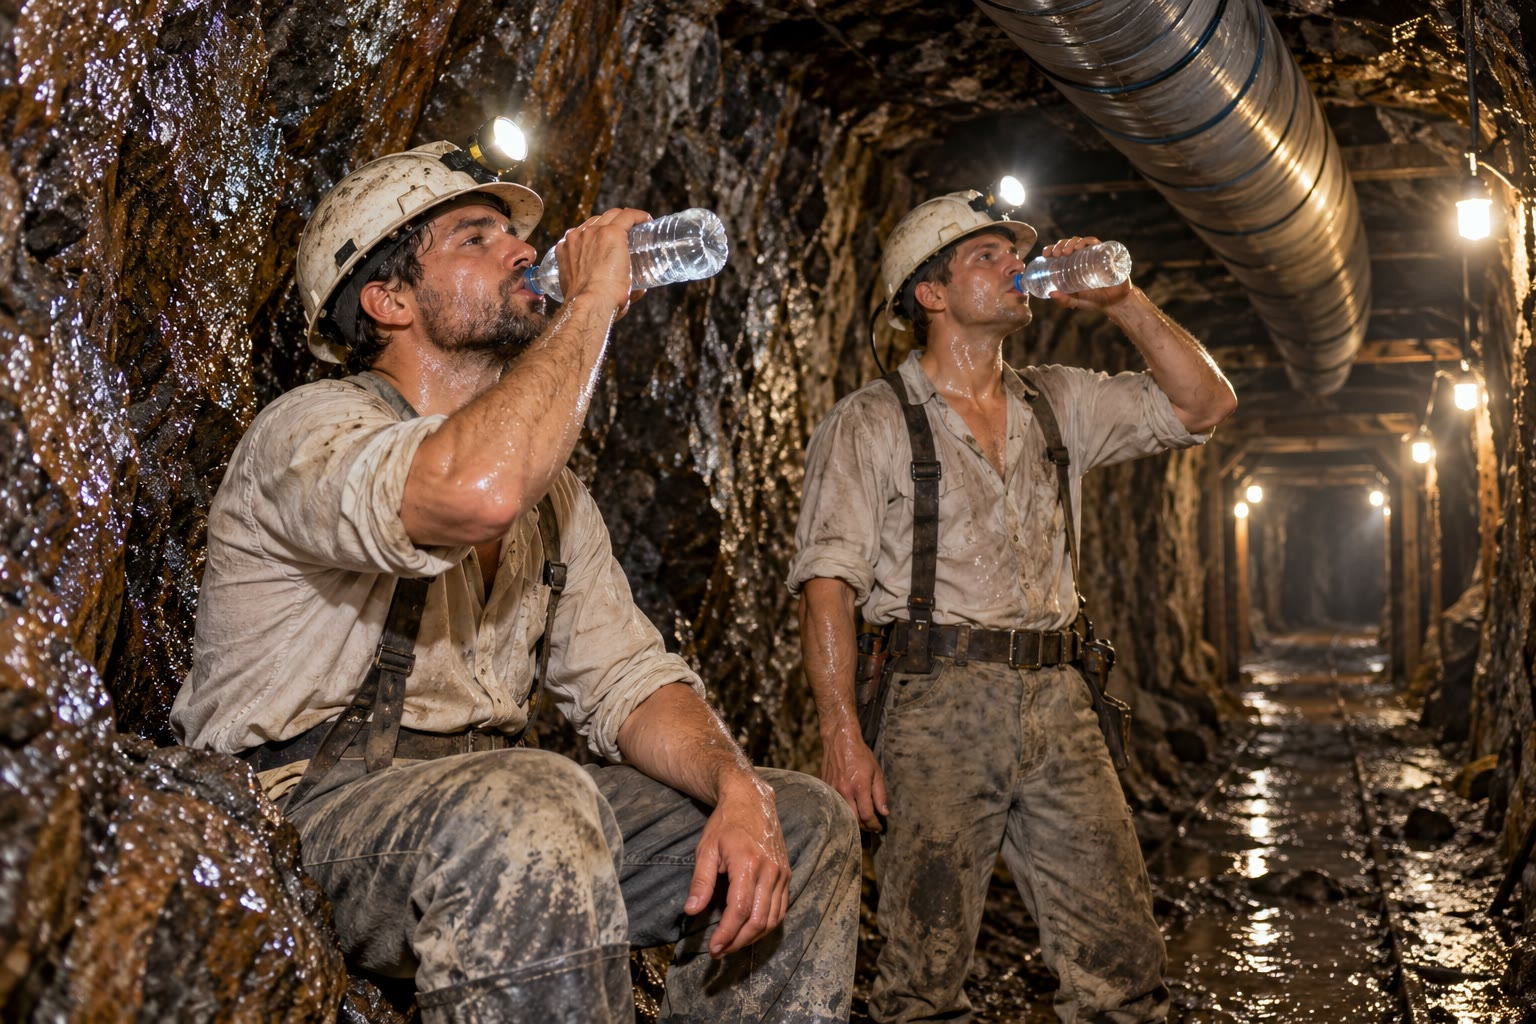
\includegraphics[width=0.62\linewidth]{images/book1/ai/g6-deep-mine.jpg}

{\small ज़मीन के किलोमीटरों नीचे एक गरम सुरंग में खनिक पानी पीते हैं।
(AI चित्रण।)}
\end{omfigure}

\begin{recall}
पृथ्वी एक \omterm{def:g6:earth-a-planet:planet-types}{चट्टानी ग्रह} है, लगभग 12\,742~km चौड़ा एक गोला: उसकी त्रिज्या, सतह से
केंद्र तक, लगभग 6371~km है
(\cref{ch:g6:earth-a-planet})। उसकी \omterm{def:g3:stones-pebbles-sand:rock}{चट्टानें} तीन परिवारों की हैं, आग्नेय,
अवसादी और कायांतरित (\cref{ch:g6:rocks-and-minerals})। \omterm{def:g4:volcanoes-earthquakes-first-look:volcano}{ज्वालामुखी} पर
पिघली \omterm{def:g3:stones-pebbles-sand:rock}{चट्टान} नीचे से ऊपर आती है और \omterm{def:g4:volcanoes-earthquakes-first-look:eruption}{लावा} बनकर बहती है; \omterm{def:g4:volcanoes-earthquakes-first-look:earthquake}{भूकंप} में ज़मीन
काँपती है (\cref{ch:g4:volcanoes-earthquakes-first-look})।
\end{recall}
% ledger: earth:Rmean

\section{हम कितनी गहराई तक गए हैं?}

लोग बहुत समय से पानी, पत्थर और धातुओं के लिए पृथ्वी में खोदते आए हैं।
दो तरह के छेद सबसे गहरे जाते हैं।

\textbf{खदानें।} दुनिया की सबसे गहरी खदान दक्षिण अफ़्रीका में जोहानिसबर्ग के पास
सोने की एक खदान है। उसकी सुरंगें सतह से 4~km से ज़्यादा नीचे जाती हैं। वहाँ
नीचे \omterm{def:g3:stones-pebbles-sand:rock}{चट्टान} की दीवारें लगभग 60~डिग्री सेल्सियस तक पहुँचती हैं: खदान को पानी में
मिली हज़ारों टन बर्फ़ नीचे पंप करके, और सुरंगों में हवा फेंकने वाले विशाल पंखों से
ठंडा किया जाता है।
% ledger: gwr:deepest-mine

\textbf{वेध-छिद्र।} वेध-छिद्र एक सँकरा छेद है जिसे एक मशीन सतह से खोदती है; उसमें
कोई नीचे नहीं जाता। सबसे गहरा वेध-छिद्र शुरुआती कहानी वाला है, जिसे रूस के
उत्तर-पश्चिम में कोला प्रायद्वीप पर विज्ञान के लिए खोदा गया:
12\,262~मीटर, यानी लगभग 12.3~km।
% ledger: sciam:kola-depth

ये गहराइयाँ बहुत बड़ी लगती हैं। पृथ्वी के आकार की तुलना में वे नन्ही हैं। नीचे
का चित्र उन्हें एक पट्टी पर दिखाता है, सबसे ऊँचे \omterm{def:g1:landscapes-around-us:landform}{पर्वत}, माउंट एवरेस्ट (8849~m), के
बगल में।
% ledger: tht:everest

\begin{omfigure}
\begin{tikzpicture}[yscale=0.27, xscale=1]
  % sea-level ground and the sky
  \fill[blue!6] (-0.2,0) rectangle (8.6,9.6);
  \fill[brown!35] (-0.2,0) rectangle (8.6,-13.4);
  \draw[thick, brown!60!black] (-0.2,0) -- (8.6,0);
  % depth axis
  \draw[->] (0,-13.4) -- (0,9.9) node[above, font=\scriptsize] {km};
  \foreach \y in {-12,-8,-4,0,4,8} \draw (-0.08,\y) -- (0.08,\y) node[left=2pt, font=\scriptsize] {\y};
  % Everest
  \fill[gray!55] (1.0,0) -- (2.2,8.849) -- (3.4,0) -- cycle;
  \draw[dashed, gray] (0,8.849) -- (2.2,8.849);
  \node[font=\scriptsize, right] at (2.35,8.6) {एवरेस्ट, 8.8~km ऊँचा};
  % deepest mine
  \draw[line width=2.2pt, black!70] (4.4,0) -- (4.4,-4);
  \draw[dashed, gray] (0,-4) -- (4.4,-4);
  \node[font=\scriptsize, right, align=left] at (4.5,-3.6) {सबसे गहरी खदान,\\ 4~km से ज़्यादा};
  % Kola borehole
  \draw[line width=0.7pt, red!75!black] (6.8,0) -- (6.8,-12.262);
  \draw[dashed, gray] (0,-12.262) -- (6.8,-12.262);
  \node[font=\scriptsize, left, align=right, red!60!black] at (6.7,-10.6) {सबसे गहरा वेध-छिद्र,\\ 12.3~km};
  % break and the centre
  \draw[white, line width=3pt] (-0.3,-13.15) -- (8.7,-12.75);
  \draw (-0.3,-13.35) -- (8.7,-12.95);
  \draw (-0.3,-12.95) -- (8.7,-12.55);
  \node[font=\footnotesize, align=center] at (4.2,-16.2) {\ldots\ और पृथ्वी का केंद्र 6371~km नीचे है:\\
     इस पट्टी पर वह इस रेखा से लगभग 17~मीटर नीचे होगा।};
\end{tikzpicture}

{\small एक ही पैमाने पर बनी ऊँचाइयाँ और गहराइयाँ (3.7~km के लिए 1~cm),
\omterm{def:g4:world-physical-map:altitude}{समुद्र तल} से। पट्टी का टूटा हुआ हिस्सा केंद्र तक का लगभग पूरा रास्ता
छिपा देता है।}
% ledger: tht:everest, gwr:deepest-mine, sciam:kola-depth, earth:Rmean
\end{omfigure}

\begin{method}[किसी गहराई की तुलना पृथ्वी की त्रिज्या से करना]\label{met:g6:inside-the-earth:percent}
\begin{enumerate}
  \item गहराई और त्रिज्या को एक ही इकाई (किलोमीटर) में लिखो।
  \item गहराई को त्रिज्या से भाग दो, फिर 100 से गुणा करो: इससे गहराई केंद्र तक
        के रास्ते के प्रतिशत के रूप में मिलती है।
  \item यह बताने के लिए कि केंद्र कितने गुना गहरा है, त्रिज्या को
        गहराई से भाग दो।
\end{enumerate}
\end{method}

\begin{example}[सबसे गहरा वेध-छिद्र]\label{ex:g6:inside-the-earth:kola}
वेध-छिद्र 12.3~km गहरा है और त्रिज्या 6371~km है।
$12.3 \div 6371 \approx 0.0019$, और $0.0019 \times 100 = 0.19$: वेध-छिद्र
केंद्र तक के रास्ते का लगभग \textbf{0.2~\%} गया। उलटी
ओर से, $6371 \div 12.3 \approx 518$: केंद्र छेद की तली से 500~गुना से भी
ज़्यादा गहरा है।

सबसे गहरी खदान के लिए, लगभग 4~km: $4 \div 6371 \approx 0.0006$, यानी
0.06~\%: वेध-छिद्र से तीन गुना कम।
% ledger: sciam:kola-depth, earth:Rmean, gwr:deepest-mine
\end{example}

इसलिए किसी ने भी पृथ्वी के गहरे भीतर को कभी देखा, छुआ या उसका नमूना नहीं लिया।
उसके बारे में हम जो जानते हैं वह दूसरे सुरागों से आता है, सबसे बढ़कर \omterm{def:g4:volcanoes-earthquakes-first-look:earthquake}{भूकंपों} की
तरंगों से (खंड~\ref{sec:g6:inside-the-earth:waves})।

\section{भूपर्पटी, प्रावार और क्रोड}

पृथ्वी परतों में बनी है, कुछ-कुछ उबले अंडे की तरह: एक पतला भुरभुरा
छिलका, एक मोटी ``सफ़ेदी'', और बीच में एक ``ज़र्दी''।
% ledger: usgs:layers-egg

\begin{omfigure}
\begin{tikzpicture}
  % a boiled egg cut in half
  \begin{scope}
    \fill[white] (0,0) ellipse (1.25 and 1.6);
    \draw[brown!50!black, line width=1.6pt] (0,0) ellipse (1.25 and 1.6);
    \fill[yellow!70!orange] (0,-0.15) circle (0.72);
    \node[font=\scriptsize, anchor=west] (s) at (1.8,1.3) {छिलका};
    \draw[gray] (s.west) -- (1.0,0.98);
    \node[font=\scriptsize, anchor=west] (w) at (1.8,0.4) {सफ़ेदी};
    \draw[gray] (w.west) -- (0.95,0.4);
    \node[font=\scriptsize, anchor=west] (y) at (1.8,-0.5) {ज़र्दी};
    \draw[gray] (y.west) -- (0.5,-0.4);
    \node[font=\small] at (0,-2.0) {एक उबला अंडा};
  \end{scope}
  \draw[->, thick, gray] (3.0,0) -- (4.2,0);
  % the Earth, not to scale
  \begin{scope}[xshift=6.2cm]
    \fill[orange!45!red!45] (0,0) circle (1.55);
    \fill[orange!75!yellow] (0,0) circle (0.95);
    \fill[yellow!55] (0,0) circle (0.42);
    \draw[brown!50!black, line width=1.6pt] (0,0) circle (1.55);
    \node[font=\scriptsize, anchor=west] (c) at (1.95,1.3) {भूपर्पटी};
    \draw[gray] (c.west) -- (1.12,1.07);
    \node[font=\scriptsize, anchor=west] (m) at (1.95,0.55) {प्रावार};
    \draw[gray] (m.west) -- (1.2,0.5);
    \node[font=\scriptsize, anchor=west] (o) at (1.95,-0.2) {बाह्य क्रोड};
    \draw[gray] (o.west) -- (0.7,-0.2);
    \node[font=\scriptsize, anchor=west] (i) at (1.95,-0.9) {आंतरिक क्रोड};
    \draw[gray] (i.west) -- (0.15,-0.25);
    \node[font=\small] at (0,-2.0) {पृथ्वी (पैमाने पर नहीं)};
  \end{scope}
\end{tikzpicture}

{\small उबले अंडे से पृथ्वी की तुलना। ज़र्दी के उलट, \omterm{def:g6:inside-the-earth:layers}{क्रोड} के
दो हिस्से हैं। इस चित्र में \omterm{def:g6:inside-the-earth:layers}{भूपर्पटी} बहुत ज़्यादा मोटी दिखाई गई है; पैमाने पर बना
चित्र आगे है।}
% ledger: usgs:layers-egg
\end{omfigure}

\begin{definition}[पृथ्वी की परतें]\label{def:g6:inside-the-earth:layers}
पृथ्वी सतह से केंद्र तक तीन मुख्य परतों से बनी है:
\begin{itemize}
  \item \emph{भूपर्पटी}\index{भूपर्पटी}, ठोस \omterm{def:g3:stones-pebbles-sand:rock}{चट्टान} की एक पतली बाहरी परत, कुछ
        किलोमीटर से कुछ दसियों किलोमीटर मोटी;
  \item \emph{प्रावार}\index{प्रावार}, गरम, घनी, ठोस \omterm{def:g3:stones-pebbles-sand:rock}{चट्टान} की एक मोटी परत,
        लगभग 2900~km की गहराई तक;
  \item \emph{क्रोड}\index{क्रोड}, धातु का बना, ज़्यादातर लोहा और थोड़ा
        निकल, लगभग 2900~km से केंद्र तक। क्रोड के दो
        हिस्से हैं: \emph{बाह्य क्रोड}\index{बाह्य क्रोड}, जो द्रव है, और
        \emph{आंतरिक क्रोड}\index{आंतरिक क्रोड}, केंद्र पर एक ठोस गोला,
        जिसकी त्रिज्या लगभग 1220~km है।
\end{itemize}
% ledger: usgs:layers-egg, usgs:crust-thickness, data:prem, earth:Rmean
\end{definition}

नीचे का चित्र परतों को \emph{पैमाने पर} दिखाता है, \omterm{def:g4:volcanoes-earthquakes-first-look:earthquake}{भूकंप} की तरंगों से नापी गई
सीमाओं के साथ।

\begin{omfigure}
\pgfplotstableread{figdata/out/grade-6-earth_layers-disc.dat}\disctab
\pgfplotstablegetelem{0}{r_cm}\of\disctab \let\rE\pgfplotsretval
\pgfplotstablegetelem{1}{r_cm}\of\disctab \let\rOC\pgfplotsretval
\pgfplotstablegetelem{2}{r_cm}\of\disctab \let\rIC\pgfplotsretval
\begin{minipage}[c]{0.43\linewidth}\centering
\begin{tikzpicture}
  \fill[orange!45!red!45] (0,0) circle (\rE cm);
  \fill[orange!75!yellow] (0,0) circle (\rOC cm);
  \fill[yellow!55] (0,0) circle (\rIC cm);
  \draw[brown!50!black, line width=0.45pt] (0,0) circle (\rE cm);
  
  \draw[gray, thin] (-0.25,\rE) rectangle (0.25,\rE-0.12);
  
  \node[font=\scriptsize, align=center, inner sep=0pt] at (0,0) {आंतरिक\\ क्रोड};
  \node[font=\scriptsize, align=center] at (0,1.03) {बाह्य\\ क्रोड};
  \node[font=\scriptsize] at (0,2.12) {प्रावार};
  \draw[<-, font=\scriptsize] (1.98,1.98) -- (2.3,2.75) node[above, align=center] {भूपर्पटी\\ (बाल जितनी पतली)};
\end{tikzpicture}
\end{minipage}\hfill
\begin{minipage}[c]{0.55\linewidth}\centering
\begin{tikzpicture}[yscale=0.034, xscale=0.55]
  % the top 100 km enlarged: ocean on the left, continent and a range on the right
  \fill[orange!45!red!45] (0,0) rectangle (12,-100);
  \fill[blue!25] (0,0) rectangle (4,-4);
  \fill[brown!45] (0,-4) rectangle (4,-9);                 % oceanic crust 5 km
  \fill[brown!60] (4,0) -- (4,-9) -- (5,-30) -- (8,-30) -- (9,-100) -- (11,-100) -- (11.4,-30) -- (12,-30) -- (12,0) -- cycle;
  \fill[brown!60] (8.6,0) -- (10,5) -- (11.4,0) -- cycle;   % the range (not to scale above ground)
  \draw[red!75!black, line width=0.8pt] (6.2,0) -- (6.2,-12.262);
  \draw[thin] (0,0) rectangle (12,-100);
  \foreach \y in {0,-20,-40,-60,-80,-100} \draw (0,\y) -- (-0.2,\y) node[left, font=\scriptsize] {\pgfmathparse{-\y}\pgfmathprintnumber{\pgfmathresult}};
  \node[font=\scriptsize, rotate=90] at (-2.0,-50) {गहराई (km)};
  \node[font=\scriptsize, align=center] at (2,-44) {महासागरीय\\ भूपर्पटी,\\ 5~km};
  \draw[->, thin] (2,-29) -- (2,-8);
  \node[font=\scriptsize, align=center] at (6.6,-21) {महाद्वीपीय\\ भूपर्पटी, 30~km};
  \node[font=\scriptsize, align=center] at (10.0,-50) {पर्वत-श्रेणी\\ की जड़,\\ 100~km\\ तक};
  \node[font=\scriptsize, align=center, red!60!black] at (7.4,-6.5) {वेध-छिद्र};
  \node[font=\scriptsize] at (4.5,-75) {प्रावार};
  \node[font=\scriptsize, blue!60!black] at (2,2.5) {महासागर};
\end{tikzpicture}
\end{minipage}

\smallskip
{\small बाएँ: पैमाने पर खुली कटी पृथ्वी; ऊपर का छोटा धूसर डिब्बा उस हिस्से को दिखाता
है जो दाईं ओर बड़ा किया गया है। दाएँ: ऊपर के 100~km, लगभग 60~गुना बड़े करके:
\omterm{def:g2:water-on-earth:ocean}{महासागरों} के नीचे पतली \omterm{def:g6:inside-the-earth:layers}{भूपर्पटी}, \omterm{def:g3:continents-and-oceans:continent}{महाद्वीपों} के नीचे मोटी \omterm{def:g6:inside-the-earth:layers}{भूपर्पटी}, ऊँची \omterm{def:g4:world-physical-map:range}{पर्वत-श्रेणियों}
के नीचे सबसे मोटी; रिकॉर्ड वेध-छिद्र लाल में।}
% ledger: data:prem, earth:Rmean, usgs:crust-thickness, sciam:kola-depth (figdata/grade-6/earth_layers.py)
\end{omfigure}

\begin{center}\small
\begin{tabular}{|l|c|c|c|l|}
\hline
\textbf{परत} & \textbf{से (km)} & \textbf{तक (km)} & \textbf{मोटाई (km)} & \textbf{किससे बनी} \\
\hline
\omterm{def:g6:inside-the-earth:layers}{भूपर्पटी} & 0 & 5 से 100 & 5 से 100 & ठोस \omterm{def:g3:stones-pebbles-sand:rock}{चट्टान} \\
\omterm{def:g6:inside-the-earth:layers}{प्रावार} & \omterm{def:g6:inside-the-earth:layers}{भूपर्पटी} की तली & 2891 & लगभग 2860 & ठोस \omterm{def:g3:stones-pebbles-sand:rock}{चट्टान}, बहुत गरम \\
\omterm{def:g6:inside-the-earth:layers}{बाह्य क्रोड} & 2891 & 5150 & लगभग 2260 & द्रव धातु \\
\omterm{def:g6:inside-the-earth:layers}{आंतरिक क्रोड} & 5150 & 6371 (केंद्र) & लगभग 1220 & ठोस धातु \\
\hline
\end{tabular}
\end{center}
% ledger: data:prem, usgs:crust-thickness, usgs:layers-egg, earth:Rmean (figdata/grade-6/earth_layers.py, main table)

\textbf{\omterm{def:g6:inside-the-earth:layers}{भूपर्पटी}} अकेली परत है जिस पर हम चल सकते हैं और जिसमें खोद सकते हैं। दूसरी
परतों की तुलना में वह बहुत पतली है: \omterm{def:g2:water-on-earth:ocean}{महासागरों} के नीचे वह केवल लगभग 5~km मोटी
है; \omterm{def:g3:continents-and-oceans:continent}{महाद्वीपों} के नीचे औसतन लगभग 30~km; आल्प्स जैसी ऊँची
\omterm{def:g4:world-physical-map:range}{पर्वत-श्रेणियों} के नीचे उसका तल 100~km तक गहरा हो सकता है, किसी दाँत की जड़ की
तरह। रिकॉर्ड वेध-छिद्र भी, 12.3~km गहरा, एक औसत महाद्वीपीय \omterm{def:g6:inside-the-earth:layers}{भूपर्पटी} के आधे से कम तक ही गया। पैमाने पर बने चित्र में \omterm{def:g6:inside-the-earth:layers}{भूपर्पटी}
चकती के चारों ओर की रेखा से भी पतली है।
% ledger: usgs:crust-thickness, sciam:kola-depth

\textbf{\omterm{def:g6:inside-the-earth:layers}{प्रावार}} सबसे मोटी परत है: वह \omterm{def:g6:inside-the-earth:layers}{भूपर्पटी} के तल से
2891~km तक जाता है, केंद्र तक के रास्ते का लगभग 45~\%। उसकी \omterm{def:g3:stones-pebbles-sand:rock}{चट्टान}
ठोस है, पर बहुत गरम और \omterm{def:g6:inside-the-earth:layers}{भूपर्पटी} की \omterm{def:g3:stones-pebbles-sand:rock}{चट्टान} से ज़्यादा घनी। लाखों
वर्षों में \omterm{def:g6:inside-the-earth:layers}{प्रावार} के एक हिस्से की गरम \omterm{def:g3:stones-pebbles-sand:rock}{चट्टान} बहुत धीरे-धीरे सरक सकती है, किसी बहुत
कड़े लेप की तरह।
% ledger: data:prem, usgs:layers-egg, usgs:lithosphere-80km

\textbf{\omterm{def:g6:inside-the-earth:layers}{क्रोड}} 2891~km पर शुरू होता है और केंद्र तक जाता है। वह
\omterm{def:g3:stones-pebbles-sand:rock}{चट्टान} से नहीं बल्कि धातु से बना है: लोहे और निकल का एक मिश्रधातु, \omterm{def:g6:inside-the-earth:layers}{प्रावार} से
लगभग दुगुना घना। उसका बाहरी हिस्सा \emph{द्रव} है: पिघली धातु का एक \omterm{def:g2:water-on-earth:ocean}{महासागर},
2000~km से ज़्यादा गहरा। उसका भीतरी हिस्सा, 5150~km से
केंद्र तक, धातु का एक \emph{ठोस} गोला है, जिसकी त्रिज्या लगभग 1220~km है: चंद्रमा की चौड़ाई का लगभग 70~\%। पृथ्वी के घूमने के साथ
\omterm{def:g6:inside-the-earth:layers}{बाह्य क्रोड} की द्रव धातु चलती है, और यह गति पृथ्वी का चुंबकीय क्षेत्र बनाती है,
वही जो दिक्सूचक की सुई को घुमाता है।
% ledger: data:prem, usgs:layers-egg, earth:Rmean, planet:Moon.diameter

जितना गहरा, उतना घना। पानी का घनत्व 1~ग्राम प्रति घन
सेंटीमीटर है: \omterm{def:g6:inside-the-earth:layers}{भूपर्पटी} की \omterm{def:g3:stones-pebbles-sand:rock}{चट्टान} उससे 2.6 से 2.9 गुना घनी है,
\omterm{def:g6:inside-the-earth:layers}{प्रावार} की तली की \omterm{def:g3:stones-pebbles-sand:rock}{चट्टान} 5~गुना से ज़्यादा, और केंद्र की धातु
लगभग 13~गुना (नीचे का आलेख देखो)। सबसे भारी पदार्थ केंद्र में हैं और सबसे हल्के ऊपर: पृथ्वी छँटी हुई है, हल्की \omterm{def:g6:inside-the-earth:layers}{भूपर्पटी} से भारी धातु के \omterm{def:g6:inside-the-earth:layers}{क्रोड} तक।
% ledger: data:prem


\begin{omfigure}
\begin{tikzpicture}
  \begin{axis}[omrecord, width=0.86\linewidth, height=5.4cm,
      xmin=0, xmax=6371, ymin=0, ymax=14,
      xlabel={सतह से नीचे गहराई (km)},
      ylabel={घनत्व (g प्रति cm$^3$)},
      xtick={0,1000,2000,3000,4000,5000,6000},
      scaled x ticks=false, x tick label style={/pgf/number format/1000 sep={}},
      clip=false]
    \fill[orange!45!red!20] (axis cs:24.4,0) rectangle (axis cs:2891,14);
    \fill[orange!75!yellow!35] (axis cs:2891,0) rectangle (axis cs:5149.5,14);
    \fill[yellow!30] (axis cs:5149.5,0) rectangle (axis cs:6371,14);
    \addplot[very thick, black] table[x=depth_km, y=rho] {figdata/out/grade-6-earth_layers-profile.dat};
    \node[font=\scriptsize] at (axis cs:1450,12.5) {प्रावार};
    \node[font=\scriptsize] at (axis cs:4020,4.5) {बाह्य क्रोड};
    \node[font=\scriptsize] at (axis cs:5760,4.5) {आंतरिक क्रोड};
    \node[font=\scriptsize, align=left, anchor=west] at (axis cs:80,1.4) {भूपर्पटी: 2.6 से 2.9};
  \end{axis}
\end{tikzpicture}

{\small हर गहराई पर पृथ्वी कितनी घनी है, \omterm{def:g4:volcanoes-earthquakes-first-look:earthquake}{भूकंप} के मापों से बने एक संदर्भ मॉडल
से। जहाँ \omterm{def:g6:inside-the-earth:layers}{प्रावार} की \omterm{def:g3:stones-pebbles-sand:rock}{चट्टान} \omterm{def:g6:inside-the-earth:layers}{क्रोड} की धातु को जगह देती है, वहाँ घनत्व लगभग 5.6 से
उछलकर लगभग 9.9~g प्रति cm$^3$ हो
जाता है।}
% ledger: data:prem (figdata/grade-6/earth_layers.py, part profile)
\end{omfigure}

\begin{inthelab}[गिलास में परतें (कक्षा में, अध्यापक के साथ)]
अध्यापक एक ऊँचे गिलास में धीरे-धीरे, एक के बाद एक, डालते हैं:
थोड़ा शहद, स्याही की एक बूँद से रंगा थोड़ा पानी, और थोड़ा खाने का तेल।
डालने का क्रम कुछ भी हो, थोड़ी देर बाद शहद तली पर, पानी
बीच में और तेल ऊपर होता है: हर द्रव हल्के द्रवों के नीचे और
घने द्रवों के ऊपर बैठ जाता है। हिलाने पर गिलास
धुँधला हो जाता है; छोड़ देने पर वह फिर से छँट जाता है। पृथ्वी भी इसी तरह परतों में बनी है: सबसे घना पदार्थ, \omterm{def:g6:inside-the-earth:layers}{क्रोड} की धातु, केंद्र में है, और सबसे हल्की \omterm{def:g3:stones-pebbles-sand:rock}{चट्टान} ऊपर।
\end{inthelab}


\begin{remark}[भूपर्पटी कितनी पतली है?]\label{rem:g6:inside-the-earth:thin-crust}
30~cm चौड़े एक स्कूली \omterm{def:g3:continents-and-oceans:globe}{ग्लोब} पर महाद्वीपीय \omterm{def:g6:inside-the-earth:layers}{भूपर्पटी} (30~km) लगभग
0.7~मिलीमीटर मोटी होगी, और महासागरीय \omterm{def:g6:inside-the-earth:layers}{भूपर्पटी} (5~km) लगभग
काग़ज़ की एक शीट जितनी मोटी। \omterm{def:g6:inside-the-earth:layers}{भूपर्पटी} त्रिज्या के एक प्रतिशत के आधे
से भी कम है: $30 \div 6371 \approx 0.0047$, यानी 0.47~\%।
% ledger: usgs:crust-thickness, earth:Rmean
\end{remark}

\section{भूकंप की तरंगें बाक़ी कैसे बताती हैं}\label{sec:g6:inside-the-earth:waves}

अगर कोई 12~km से ज़्यादा गहरा नहीं गया, तो हम \omterm{def:g6:inside-the-earth:layers}{क्रोड} का चित्र कैसे बना सकते हैं? जवाब
\omterm{def:g4:volcanoes-earthquakes-first-look:earthquake}{भूकंपों} से आता है। जब \omterm{def:g4:volcanoes-earthquakes-first-look:earthquake}{भूकंप} ज़मीन को हिलाता है, तो तरंगें उससे सभी दिशाओं में
निकलती हैं और पूरी पृथ्वी के \emph{आर-पार} जाती हैं, जैसे किसी दस्तक की आवाज़ दीवार
के आर-पार जाती है। दुनिया भर में बहुत-सी जगहों पर यंत्र दर्ज करते हैं कि हर तरंग कब पहुँचती है (तुम उनसे
\cref{ch:g7:earthquakes} में मिलोगे)।
% ledger: data:prem

तरंगें हर पदार्थ में एक ही चाल से नहीं चलतीं। जब वे दो परतों की सीमा पर पहुँचती
हैं, तो उनकी चाल अचानक बदल जाती है: कुछ तरंगें लौट आती हैं, कुछ पार करते हुए
मुड़ जाती हैं, कुछ-कुछ पानी में घुसते प्रकाश की तरह। पूरे \omterm{def:g3:continents-and-oceans:globe}{ग्लोब} पर फैले केंद्रों पर बहुत-से \omterm{def:g4:volcanoes-earthquakes-first-look:earthquake}{भूकंपों} की तरंगों का समय नापकर वैज्ञानिकों ने पता किया है कि ये सीमाएँ कहाँ हैं, और
कौन-सी परतें ठोस हैं और कौन-सी द्रव। भूकंपविज्ञानी तरंगों की दो मुख्य क़िस्मों को
\emph{P तरंगें} (तेज़ वाली, जो \omterm{def:g3:stones-pebbles-sand:rock}{चट्टान} को धकेलती और खींचती हैं) और
\emph{S तरंगें} (धीमी वाली, जो उसे एक ओर से दूसरी ओर हिलाती हैं) कहते हैं; आगे के
खंड उनका बारीकी से अध्ययन करते हैं। S तरंगों का एक अनोखा गुण है: वे
किसी द्रव में से नहीं गुज़र सकतीं।

\begin{omfigure}
\begin{tikzpicture}
  \begin{axis}[omrecord, width=0.86\linewidth, height=5.4cm,
      xmin=0, xmax=6371, ymin=0, ymax=14.5,
      xlabel={सतह से नीचे गहराई (km)},
      ylabel={तरंग की चाल (km प्रति सेकंड)},
      xtick={0,1000,2000,3000,4000,5000,6000},
      scaled x ticks=false, x tick label style={/pgf/number format/1000 sep={}},
      clip=false]
    \fill[orange!45!red!20] (axis cs:24.4,0) rectangle (axis cs:2891,14.5);
    \fill[orange!75!yellow!35] (axis cs:2891,0) rectangle (axis cs:5149.5,14.5);
    \fill[yellow!30] (axis cs:5149.5,0) rectangle (axis cs:6371,14.5);
    \addplot[very thick, blue!70!black] table[x=depth_km, y=vp] {figdata/out/grade-6-earth_layers-profile.dat};
    \addplot[very thick, red!75!black] table[x=depth_km, y=vs] {figdata/out/grade-6-earth_layers-profile.dat};
    \node[font=\scriptsize, blue!70!black, anchor=south] at (axis cs:1300,12.9) {P तरंगें (तेज़)};
    \node[font=\scriptsize, red!75!black, anchor=north] at (axis cs:1500,6.1) {S तरंगें (धीमी)};
    \node[font=\scriptsize, red!75!black, align=center, fill=white, fill opacity=0.8, text opacity=1] at (axis cs:4020,1.9) {S तरंगें: 0\\ (द्रव)};
    \node[font=\scriptsize] at (axis cs:4020,13.6) {बाह्य क्रोड};
    \node[font=\scriptsize] at (axis cs:5760,13.6) {आंतरिक क्रोड};
    \node[font=\scriptsize] at (axis cs:1450,1.5) {प्रावार};
  \end{axis}
\end{tikzpicture}

{\small उसी संदर्भ मॉडल में हर गहराई पर \omterm{def:g4:volcanoes-earthquakes-first-look:earthquake}{भूकंप} की दोनों तरह की तरंगों की चाल।
\omterm{def:g6:inside-the-earth:layers}{बाह्य क्रोड} में S तरंगें रुक जाती हैं: उनकी चाल
शून्य है, क्योंकि \omterm{def:g6:inside-the-earth:layers}{बाह्य क्रोड} द्रव है।}
% ledger: data:prem (figdata/grade-6/earth_layers.py, part profile)
\end{omfigure}

आलेख को बाएँ से दाएँ पढ़ो: \omterm{def:g6:inside-the-earth:layers}{प्रावार} में दोनों तरह की तरंगें
गहराई के साथ तेज़ और तेज़ चलती हैं। 2891~km पर S तरंगें ग़ायब हो जाती हैं और
P तरंगें अचानक धीमी हो जाती हैं: यह द्रव \omterm{def:g6:inside-the-earth:layers}{बाह्य क्रोड} का ऊपरी सिरा है।
5150~km पर P तरंगें फिर तेज़ होती हैं और S तरंगें फिर से होती हैं: यह
ठोस \omterm{def:g6:inside-the-earth:layers}{आंतरिक क्रोड} है।
% ledger: data:prem

\begin{history}[इंगे लेहमान और आंतरिक क्रोड]
\begin{minipage}[c]{0.72\linewidth}
1930 के दशक की शुरुआत में भूकंपविज्ञानी सोचते थे कि पृथ्वी की दो परतें हैं: एक द्रव \omterm{def:g6:inside-the-earth:layers}{क्रोड} के चारों ओर एक ठोस \omterm{def:g6:inside-the-earth:layers}{प्रावार}। डेनमार्क की भूकंपविज्ञानी इंगे लेहमान ने
1929 में न्यूज़ीलैंड में आए एक तेज़ \omterm{def:g4:volcanoes-earthquakes-first-look:earthquake}{भूकंप} की तरंगों का अध्ययन किया, जिन्हें दूर-दूर
के केंद्रों ने दर्ज किया था। कुछ तरंगें वहाँ पहुँचीं जहाँ, पूरी तरह द्रव \omterm{def:g6:inside-the-earth:layers}{क्रोड}
के लिए, उन्हें पहुँचना ही नहीं चाहिए था। 1936 के एक लेख में, जिसका नाम बस ``P\,$'$'' था,
उन्होंने एक व्याख्या रखी: द्रव \omterm{def:g6:inside-the-earth:layers}{क्रोड} के भीतर एक छोटा
\emph{ठोस \omterm{def:g6:inside-the-earth:layers}{आंतरिक क्रोड}} है, जो इन तरंगों को लौटा देता है। उन्होंने विनम्रता से लिखा
कि आँकड़े निश्चित होने के लिए ``काफ़ी अपर्याप्त'' थे, पर यह
व्याख्या ``संभव लगती है'', और उन्होंने दूसरे शोधकर्ताओं से उसे परखने को कहा।
उन्होंने परखा, और आज ठोस \omterm{def:g6:inside-the-earth:layers}{आंतरिक क्रोड} पृथ्वी के हर संदर्भ मॉडल का हिस्सा है, जैसे इस अध्याय के आलेखों में प्रयुक्त मॉडल।
% ledger: nbi:lehmann-1936
\end{minipage}\hfill
\begin{minipage}[c]{0.24\linewidth}\centering
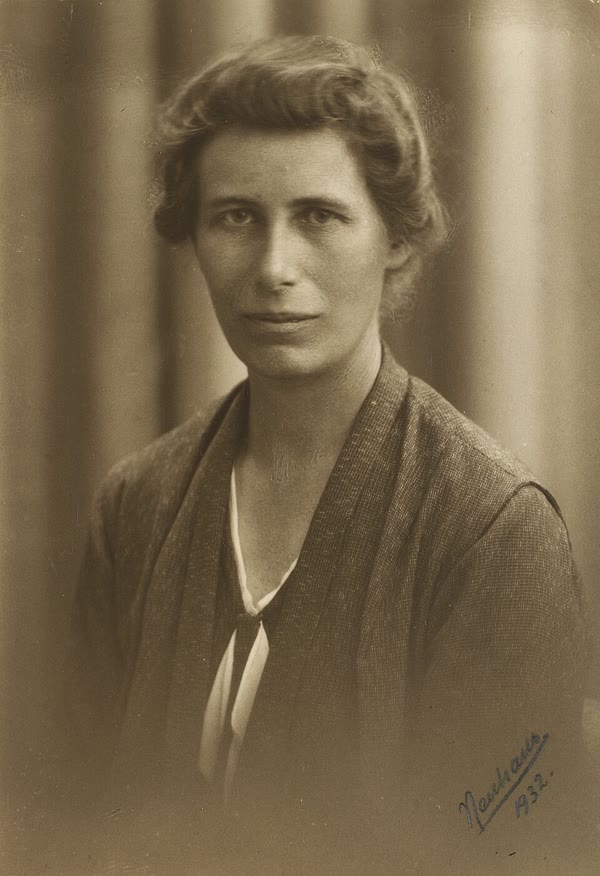
\includegraphics[width=\linewidth]{images/book1/g6-inge-lehmann.jpg}\\[2pt]
{\footnotesize 1932 में इंगे लेहमान। (फ़ोटो: इवन नॉयहाउस, सार्वजनिक डोमेन,
विकिमीडिया कॉमन्स के ज़रिए।)}
% ledger: commons:inge-lehmann
\end{minipage}
\end{history}

\section{जितना गहरा, उतना गरम}

हर गहरी खदान और हर गहरा वेध-छिद्र एक ही बात दिखाता है: जितना गहरा
जाओ, \omterm{def:g3:stones-pebbles-sand:rock}{चट्टान} उतनी गरम। सबसे गहरी खदान में \omterm{def:g3:stones-pebbles-sand:rock}{चट्टान} की दीवारें 4~km से ज़्यादा नीचे
लगभग 60~डिग्री सेल्सियस तक पहुँचती हैं; रिकॉर्ड वेध-छिद्र की तली पर,
12.3~km नीचे, \omterm{def:g3:stones-pebbles-sand:rock}{चट्टान} लगभग 180~डिग्री पर थी।
% ledger: gwr:deepest-mine, sciam:kola-180C

सतह के पास तापमान एक काफ़ी स्थिर दर से बढ़ता है। संयुक्त
राज्य अमेरिका में वैज्ञानिकों ने 284 वेध-छिद्रों के माप इकट्ठा किए, जिनमें से
ज़्यादातर 600~m से गहरे थे। औसतन तापमान गहराई के हर किलोमीटर पर
\textbf{29~डिग्री} बढ़ा: देश के पूर्व में लगभग 25~डिग्री प्रति
किलोमीटर और पश्चिम में 34। पर यह दर जगह-जगह बहुत बदलती है: उन छेदों में वह
6 से 69~डिग्री प्रति किलोमीटर तक थी।
% ledger: usgs:gradient-29

\begin{omfigure}
\begin{tikzpicture}
  \begin{axis}[omrecord, omdepth, width=0.78\linewidth, height=5.6cm,
      xmin=0, xmax=160, ymin=0, ymax=2,
      xlabel={चट्टान का तापमान ($^\circ$C)},
      ylabel={गहराई (km)},
      ytick={0,0.5,1,1.5,2},
      yticklabel style={/pgf/number format/fixed},
      legend pos=north east, legend cell align=left,
            legend style={font=\scriptsize},
      clip=false]
    \addplot[forget plot, name path=lo, thin, gray] table[x=t_low, y=depth_km] {figdata/out/grade-6-earth_layers-geotherm.dat};
    \addplot[forget plot, name path=hi, thin, gray] table[x=t_high, y=depth_km] {figdata/out/grade-6-earth_layers-geotherm.dat};
    \addplot[forget plot, gray!20] fill between[of=lo and hi];
    \addplot[forget plot, thick, blue!70!black] table[x=t_east, y=depth_km] {figdata/out/grade-6-earth_layers-geotherm.dat};
    \addplot[forget plot, very thick, black] table[x=t_mean, y=depth_km] {figdata/out/grade-6-earth_layers-geotherm.dat};
    \addplot[forget plot, thick, red!75!black] table[x=t_west, y=depth_km] {figdata/out/grade-6-earth_layers-geotherm.dat};
    \addlegendimage{area legend, fill=gray!20, draw=gray}
    \addlegendentry{6 से 69 $^\circ$C प्रति km: सभी छेद}
    \addlegendimage{thick, blue!70!black}\addlegendentry{25 $^\circ$C प्रति km: पूर्व}
    \addlegendimage{very thick, black}\addlegendentry{29 $^\circ$C प्रति km: औसत}
    \addlegendimage{thick, red!75!black}\addlegendentry{34 $^\circ$C प्रति km: पश्चिम}
  \end{axis}
\end{tikzpicture}

{\small 15~$^\circ$C से शुरू होने वाली ज़मीन के लिए गहराई (नीचे की ओर) के साथ तापमान,
औसत दर (29, काली), पूर्वी और पश्चिमी
औसत (25 और 34) और नापी गई पूरी सीमा (6 से 69, धूसर पट्टी) पर। माप
लगभग 2~km तक जाते हैं।}
% ledger: usgs:gradient-29, planet:Earth.Tmean (figdata/grade-6/earth_layers.py, part geotherm)
\end{omfigure}

\begin{method}[किसी गहराई पर तापमान]\label{met:g6:inside-the-earth:temperature}
\begin{enumerate}
  \item सतह के पास ज़मीन का तापमान लो।
  \item गहराई को, किलोमीटर में, दर से, डिग्री प्रति
        किलोमीटर में, गुणा करो: इतना ज़्यादा गरम हो जाता है।
  \item दोनों को जोड़ो। इसका प्रयोग केवल उस सीमा में करो जहाँ दर
        नापी गई थी: कुछ किलोमीटर।
\end{enumerate}
\end{method}

\begin{example}[दो किलोमीटर नीचे]\label{ex:g6:inside-the-earth:two-km}
ज़मीन 15~$^\circ$C पर है और दर 29~डिग्री प्रति किलोमीटर है।
2~km पर: $2 \times 29 = 58$ डिग्री ज़्यादा गरम, इसलिए $15 + 58 = 73~^\circ$C:
सबसे गरम स्नान से भी गरम, और छूने के लिए पहले से बहुत ज़्यादा गरम।
% ledger: usgs:gradient-29, planet:Earth.Tmean
\end{example}

क्या यही दर केंद्र तक काम में ली जा सकती है? नहीं। 29~डिग्री प्रति
किलोमीटर पर केंद्र लगभग 185\,000~डिग्री पर होता, जो
असंभव है: पहले किलोमीटरों में नापी गई दर बहुत नीचे लागू नहीं होती, जहाँ बढ़त बहुत धीमी होनी चाहिए। वैज्ञानिक \omterm{def:g6:inside-the-earth:layers}{क्रोड} के तापमान का
अनुमान दूसरे ढंग से लगाते हैं: प्रयोगशाला में वे लोहे के नन्हे कणों को दो हीरों के
बीच, हवा के दाब के लाखों गुना तक दबाते हैं,
और उन्हें लेज़र से तब तक गरम करते हैं जब तक वे पिघल न जाएँ। इस तरह उन्होंने पाया कि
ठोस \omterm{def:g6:inside-the-earth:layers}{आंतरिक क्रोड} के किनारे पर तापमान लगभग
\textbf{6000~डिग्री सेल्सियस} है, और फिर भी \omterm{def:g6:inside-the-earth:layers}{आंतरिक क्रोड} का लोहा ठोस रहता है, क्योंकि वहाँ का दाब, हवा के दाब का लगभग
33~लाख गुना, उसे पिघलने से रोकता है।
% ledger: esrf:core-6000C, usgs:gradient-29

\begin{remark}[गरम, फिर भी ठोस]\label{rem:g6:inside-the-earth:pressure}
किसी पदार्थ को ज़ोर से दबाने पर वह केवल ज़्यादा ऊँचे तापमान पर पिघलता है।
\omterm{def:g6:inside-the-earth:layers}{प्रावार} बहुत गरम है, फिर भी ठोस रहता है; \omterm{def:g6:inside-the-earth:layers}{बाह्य क्रोड} द्रव है; \omterm{def:g6:inside-the-earth:layers}{आंतरिक
क्रोड}, और भी गरम, फिर से ठोस है, क्योंकि उसे सबसे ज़्यादा दबाया जाता है।
कोई चीज़ पिघलती है या नहीं, यह तापमान \emph{और} दाब पर निर्भर करता है।
% ledger: esrf:core-6000C, data:prem
\end{remark}

\section{अभ्यास}

\begin{exercise}[$\star$]\label{exo:g6:inside-the-earth:1}
पृथ्वी की चारों परतों के नाम क्रम से बताओ, सतह से
केंद्र तक। कौन-सी द्रव है? कौन-सी धातु की बनी हैं?
\end{exercise}

\begin{exercise}[$\star$]\label{exo:g6:inside-the-earth:2}
सही या ग़लत? ग़लत वाक्यों को सुधारो।
(क) \omterm{def:g6:inside-the-earth:layers}{भूपर्पटी} \omterm{def:g3:continents-and-oceans:continent}{महाद्वीपों} के नीचे की तुलना में \omterm{def:g2:water-on-earth:ocean}{महासागरों} के नीचे ज़्यादा मोटी है।
(ख) \omterm{def:g6:inside-the-earth:layers}{क्रोड} \omterm{def:g3:stones-pebbles-sand:rock}{चट्टान} का बना है।
(ग) \omterm{def:g6:inside-the-earth:layers}{आंतरिक क्रोड} ठोस है।
(घ) अब तक खोदा गया सबसे गहरा वेध-छिद्र लगभग 12~km गहरा है।
\end{exercise}

\begin{exercise}[$\star$]\label{exo:g6:inside-the-earth:3}
परतों की तालिका का प्रयोग करो। (क) \omterm{def:g6:inside-the-earth:layers}{क्रोड} किस गहराई पर शुरू होता है?
(ख) \omterm{def:g6:inside-the-earth:layers}{आंतरिक क्रोड} किस गहराई पर शुरू होता है? (ग) \omterm{def:g6:inside-the-earth:layers}{बाह्य क्रोड} कितना
मोटा है?
\end{exercise}

\begin{exercise}[$\star$]\label{exo:g6:inside-the-earth:4}
पृथ्वी की तुलना अक्सर उबले अंडे से की जाती है। उतारो और पूरा करो: ``छिलका
\ldots{} जैसा है, सफ़ेदी \ldots{} जैसी है और ज़र्दी
\ldots{} जैसी है। पर ज़र्दी के उलट, \ldots{} के दो हिस्से हैं: एक द्रव
\ldots{} और एक ठोस \ldots{}।''
\end{exercise}

\begin{exercise}[$\star\star$]\label{exo:g6:inside-the-earth:5}
माउंट एवरेस्ट 8.849~km ऊँचा है और पृथ्वी की त्रिज्या 6371~km है। त्रिज्या के
प्रतिशत के रूप में एवरेस्ट कितना ऊँचा है? दशमलव के दो स्थानों तक पूर्णांकित करो।
क्या दूर से देखने पर पृथ्वी की सतह बहुत ऊबड़-खाबड़ है?
\end{exercise}

\begin{exercise}[$\star\star$]\label{exo:g6:inside-the-earth:6}
महाद्वीपीय \omterm{def:g6:inside-the-earth:layers}{भूपर्पटी} औसतन 30~km मोटी है और महासागरीय \omterm{def:g6:inside-the-earth:layers}{भूपर्पटी}
5~km। (क) महाद्वीपीय \omterm{def:g6:inside-the-earth:layers}{भूपर्पटी} कितने गुना मोटी है? (ख) किसी ऊँची
\omterm{def:g4:world-physical-map:range}{पर्वत-श्रेणी} के नीचे \omterm{def:g6:inside-the-earth:layers}{भूपर्पटी} 100~km तक पहुँच सकती है। यह महासागरीय \omterm{def:g6:inside-the-earth:layers}{भूपर्पटी} से
कितने गुना मोटी है?
\end{exercise}

\begin{exercise}[$\star\star$]\label{exo:g6:inside-the-earth:7}
किसी क्षेत्र में ज़मीन 12~$^\circ$C पर है और तापमान हर किलोमीटर पर
25~डिग्री बढ़ता है। तापमान क्या है (क) 1~km पर, (ख)
1.5~km पर, (ग) 2~km पर?
\end{exercise}

\begin{exercise}[$\star\star$]\label{exo:g6:inside-the-earth:8}
किसी वेध-छिद्र में \omterm{def:g3:stones-pebbles-sand:rock}{चट्टान} सतह के पास 14~$^\circ$C पर है और
2~km की गहराई पर 74~$^\circ$C पर। हर किलोमीटर पर तापमान कितने डिग्री
बढ़ता है? क्या यह दर अध्याय के मापों के पूर्वी और पश्चिमी
औसतों के बीच है?
\end{exercise}

\begin{exercise}[$\star\star$]\label{exo:g6:inside-the-earth:9}
तरंगों की चाल के आलेख का प्रयोग करो। (क) \omterm{def:g6:inside-the-earth:layers}{क्रोड} के ठीक ऊपर, लगभग 2890~km पर, और
\omterm{def:g6:inside-the-earth:layers}{क्रोड} के ऊपरी सिरे के ठीक नीचे P तरंगों की चाल क्या है?
(ख) किन गहराइयों के बीच S तरंगों की चाल शून्य है? (ग) इससे हमें
उस परत के बारे में क्या पता चलता है?
\end{exercise}

\begin{exercise}[$\star\star$]\label{exo:g6:inside-the-earth:10}
रिकॉर्ड वेध-छिद्र 12.3~km गहरा है। (क) उसने एक औसत
महाद्वीपीय \omterm{def:g6:inside-the-earth:layers}{भूपर्पटी} (30~km) का कितना प्रतिशत पार किया? (ख) क्या वह \omterm{def:g6:inside-the-earth:layers}{प्रावार} तक पहुँचा?
\end{exercise}

\begin{exercise}[$\star\star\star$]\label{exo:g6:inside-the-earth:11}
लियो कहता है: ``सतह के पास तापमान हर किलोमीटर पर 29~डिग्री बढ़ता है,
इसलिए केंद्र पर, 6371~km नीचे, वह
$15 + 29 \times 6371$ डिग्री होना चाहिए।'' (क) लियो की संख्या निकालो। (ख) उसकी तुलना
\omterm{def:g6:inside-the-earth:layers}{आंतरिक क्रोड} के किनारे के लिए प्रयोगशाला में पाए गए तापमान से करो। (ग) लियो के तर्क
में क्या ग़लत है?
\end{exercise}

\begin{exercise}[$\star\star\star$]\label{exo:g6:inside-the-earth:12}
पूरी पृथ्वी का औसत घनत्व लगभग 5.5~ग्राम प्रति घन
सेंटीमीटर है (\cref{ch:g6:earth-a-planet}), पर \omterm{def:g6:inside-the-earth:layers}{भूपर्पटी} की \omterm{def:g3:stones-pebbles-sand:rock}{चट्टानों} का
घनत्व केवल 2.6 से 2.9 है। (क) इससे हमें और गहरे के पदार्थ के बारे में क्या पता
चलता है? (ख) घनत्व के आलेख का प्रयोग करो: किन परतों में घनत्व हर जगह 5.5 से ज़्यादा है? (ग) भारी धातु का केंद्र में, और सतह पर नहीं,
होना समझदारी की बात क्यों है?
\end{exercise}

\section{समस्या: केंद्र तक की यात्रा, पैमाने पर}

\begin{problem}[{सप्ताहांत समस्या --- 2~मीटर चौड़ी एक मॉडल पृथ्वी: परतें, सबसे
गहरे छेद और गरम भीतर, पैमाने पर बने}]
\label{pb:g6:inside-the-earth:1}
% ledger: earth:Rmean, data:prem, usgs:crust-thickness, sciam:kola-depth, tht:everest, usgs:gradient-29, gwr:deepest-mine, esrf:core-6000C
स्कूल के मेले के लिए एक कक्षा आधी कटी पृथ्वी का एक मॉडल बनाती है, जितना
बड़ा हो सके: आधे गोले का समतल फलक 2~मीटर चौड़ी एक चकती है,
जिस पर परतें रँगी हैं। सब कुछ पैमाने पर होना चाहिए। इनका प्रयोग करो: पृथ्वी की
त्रिज्या 6371~km; \omterm{def:g6:inside-the-earth:layers}{बाह्य क्रोड} का ऊपरी सिरा 2891~km; \omterm{def:g6:inside-the-earth:layers}{आंतरिक क्रोड} का ऊपरी सिरा
5150~km; महाद्वीपीय \omterm{def:g6:inside-the-earth:layers}{भूपर्पटी} 30~km; महासागरीय \omterm{def:g6:inside-the-earth:layers}{भूपर्पटी} 5~km; एवरेस्ट 8.849~km;
रिकॉर्ड वेध-छिद्र 12.3~km।

\medskip
\noindent\textbf{भाग I --- मॉडल।}
\begin{enumerate}
  \item पृथ्वी का व्यास, किलोमीटर में, क्या है? मॉडल का
        व्यास मिलीमीटर में लिखो।
  \item मॉडल का 1~मिलीमीटर असली पृथ्वी के कितने किलोमीटर के बराबर है?
        (असली व्यास को मॉडल के व्यास से भाग दो।)
  \item मॉडल पर एवरेस्ट कितना ऊँचा है, मिलीमीटर में? दशमलव के एक
        स्थान तक पूर्णांकित करो।
  \item मॉडल पर रिकॉर्ड वेध-छिद्र कितना गहरा है? उसकी तुलना मॉडल की सतह से
        केंद्र तक की दूरी से करो।
\end{enumerate}

\medskip
\noindent\textbf{भाग II --- परतें।}
\begin{enumerate}[resume]
  \item मॉडल की सतह से कितनी दूरी नीचे विद्यार्थियों को \omterm{def:g6:inside-the-earth:layers}{बाह्य क्रोड} का ऊपरी
        सिरा रँगना चाहिए? निकटतम मिलीमीटर तक पूर्णांकित करो।
  \item \omterm{def:g6:inside-the-earth:layers}{आंतरिक क्रोड} के ऊपरी सिरे के लिए वही प्रश्न। मॉडल पर \omterm{def:g6:inside-the-earth:layers}{आंतरिक क्रोड} की
        त्रिज्या क्या है?
  \item मॉडल की एक त्रिज्या के साथ कौन-सी परत सबसे ज़्यादा जगह घेरती है:
        \omterm{def:g6:inside-the-earth:layers}{प्रावार}, \omterm{def:g6:inside-the-earth:layers}{बाह्य क्रोड} या \omterm{def:g6:inside-the-earth:layers}{आंतरिक क्रोड}? मॉडल पर उसकी मोटाई
        बताओ।
  \item महाद्वीपीय \omterm{def:g6:inside-the-earth:layers}{भूपर्पटी} कितनी मोटी रँगी जानी चाहिए? दशमलव के एक
        स्थान तक पूर्णांकित करो। क्या ब्रश से यह आसान है?
\end{enumerate}

\medskip
\noindent\textbf{भाग III --- गरम भीतर।}
\begin{enumerate}[resume]
  \item विद्यार्थी 2~km पर तापमान लिखते हैं, 15~$^\circ$C की ज़मीन और
        29~डिग्री प्रति किलोमीटर लेकर। वे क्या लिखते हैं? मॉडल की
        सतह से कितनी दूरी नीचे 2~km है?
  \item सबसे गहरी खदान 4~km से ज़्यादा नीचे जाती है। मॉडल पर खदान रिकॉर्ड
        वेध-छिद्र से गहरी है या उथली? लगभग कितने
        मिलीमीटर?
  \item \omterm{def:g6:inside-the-earth:layers}{आंतरिक क्रोड} के किनारे के पास लेबल पर लिखा है ``लगभग
        6000~$^\circ$C, ठोस''। एक दर्शक हैरान है: \omterm{def:g6:inside-the-earth:layers}{बाह्य क्रोड}
        द्रव क्यों है पर \omterm{def:g6:inside-the-earth:layers}{आंतरिक क्रोड}, जो और भी गरम है, ठोस?
  \item महासागरीय \omterm{def:g6:inside-the-earth:layers}{भूपर्पटी} सबसे पतली परत है। मॉडल पर वह कितनी मोटी होनी चाहिए,
        मिलीमीटर में? दशमलव के दो स्थानों तक पूर्णांकित करो, और उसकी तुलना
        काग़ज़ की एक शीट की मोटाई (लगभग 0.1~mm) से करो।
\end{enumerate}
\end{problem}
